\chapter{Research Methodology}

\section{Methodological approach}

\paragraph{}
The aim of this research is to address a theoretical research problem. Since  graph summarization techniques have to be evaluated and benchmarked against each other, quantitative methods best suit this research. Internal validity of the research can be ensured as the causal relationship that will be tested is trustworthy and not influenced by any other factors. Since this is an algorithmic kind of research, the ideal experimentation environment can be almost similar to a real world scenario. Therefore the external validity of the research can be ensured as well. 

\section{Methods of data collection}

\paragraph{}
For this research, mostly large real world graphs will be used. These datasets can belong to different application domains such as social networks, network packet routes or even a citation network. When selecting the datasets an extra effort was taken to ensure that they are as different from each other as possible. 

\paragraph{}
The experiments will consist of testing the graph summarization algorithms with the collected data and measuring various aspects such as memory consumption, average error against each other. 

\section{Methods of analysis}

\paragraph{}
Quantitative analysis methods will be used when analyzing the results obtained by running different sketching algorithms on obtained datasets. This research belongs to the experimental type as indicated in Figure \ref{figure:design}. 

\begin{figure}[H]
    \centering
    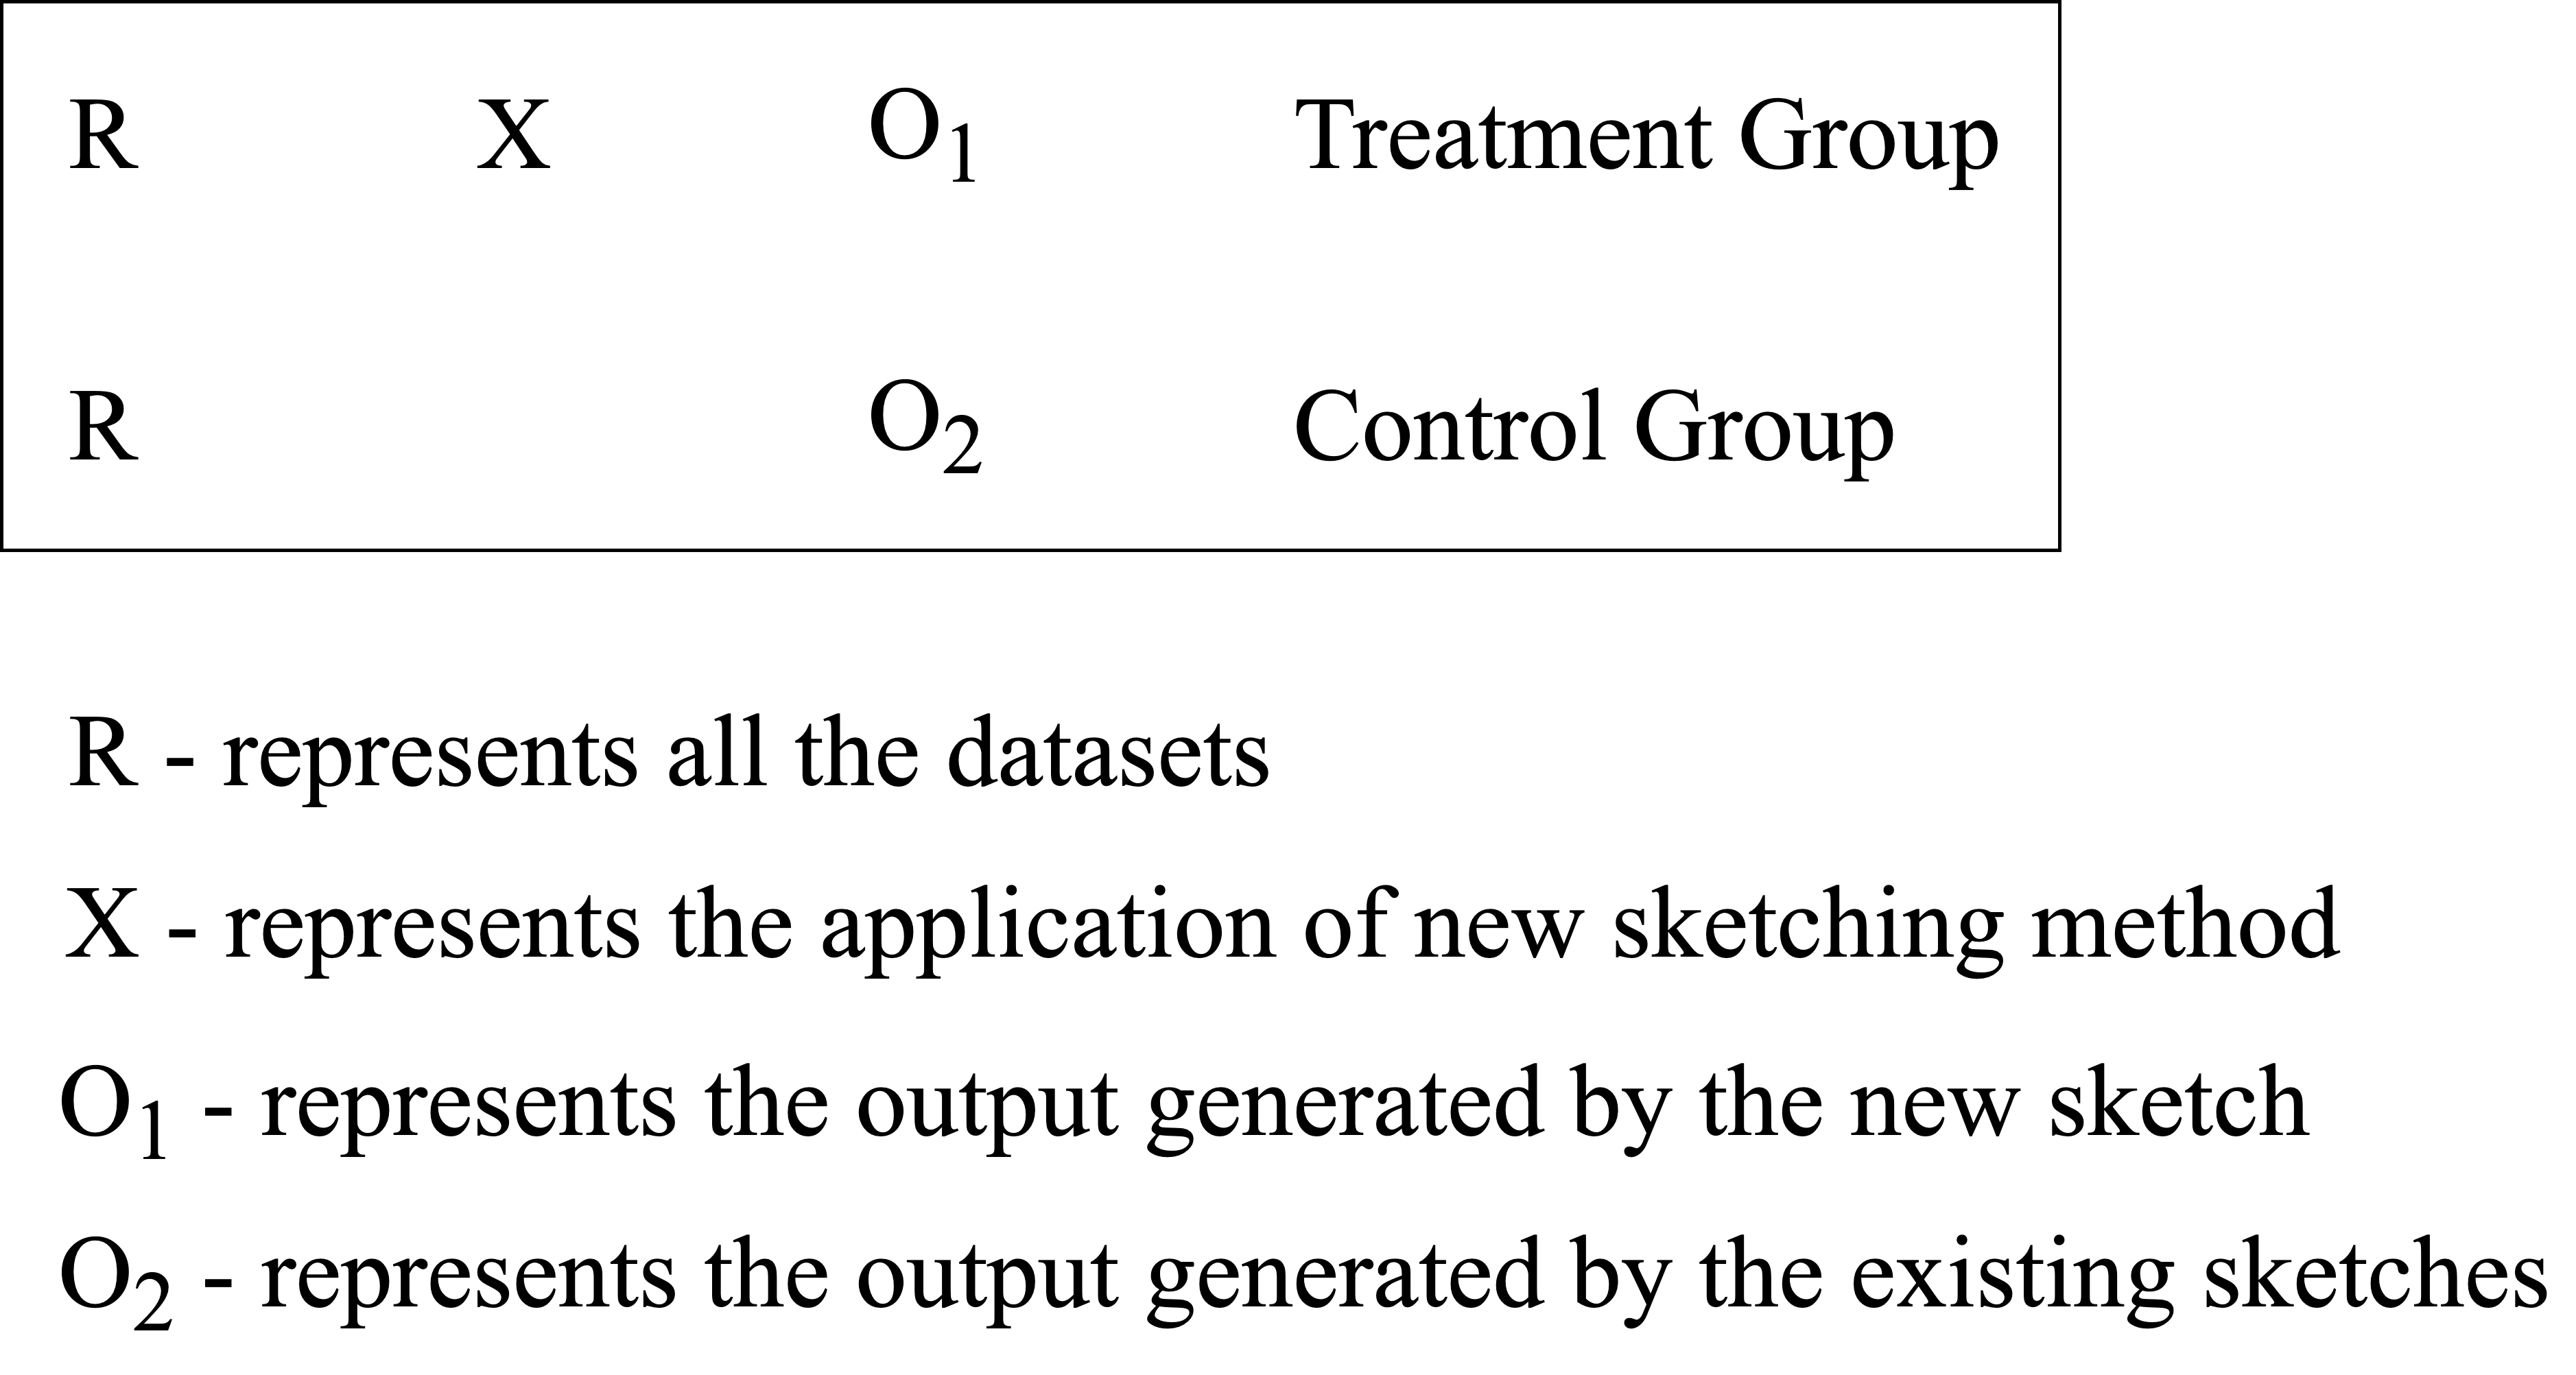
\includegraphics[width=0.6\textwidth]{images/design}
    \caption{Research design}
    \label{figure:design}
\end{figure}